\section{Further extensions}

\subsection{Estimator selection}

((Estimator selection involves actively fitting the best model as opposed to
``checking'' a numerical model that’s been given. This problem is more difficult
to define, and the value that the visualization system adds is not as concrete
))

\subsection{Outlier removal}

((Outliers are unavoidable in raw data and can skew results quite a bit. When
can the system remove outliers? What criteria should it use? ))

\subsection{Edge-weighted graphs}

(( This is more of an extension on graphical models, but it is still related to
estimator selection. In an edge-weighted graph, edges can be weighted depending
on the type of conditional dependence – negative or positive, assign 1 or -1. 0
(no edge) still implies conditional independence ))

\subsection{Regression and graphical models}

A single correlation can be thought of as a regression of the response variable
against only one observed variable; it is a ``local'' property because it
compares the behavior of only two random variables. On the other hand, a single
link in a graphical model can be thought of as a regression of the response
variable against all variables in the space. It is more nuanced than that, but
the idea is that a graphical model has a “global” property because it takes all
of the other variables into account. Although it may seem simple to numerically
quantify the dependencies with correlation as conditional dependencies are less
intuitive to compute, correlations tend to fall short of the desired result due
to the property of transitivity.

As mentioned earlier, we would like to find stocks that are as uncorrelated as
possible in order to achieve the most robust portfolio. A common methodology to
do this is to forego plotting entirely and numerically compute the correlation
matrix then create a graph from that. By construction, the correlation matrix
applies the same correlation computation to each set of observed and response
variables. Correlation coefficients are rather limited and have their own flaws,
so no coefficient is a “one size fits all” solution. For example, some variables
could share a linear relationship with the response (ideal for a Pearson
correlation) while others may not. While on the subject of the Pearson
correlation, it should be noted that correlation graphs are still interesting
because two variables that have a correlation coefficient near 0 may not
necessarily be uncorrelated. A visualization tool can reveal this by showing
outliers or patterns in the data that the analyst wasn't expecting
(Section~\ref{sec:intro:me2}). Thus, the analyst needs to perform a visual check
of the resulting correlation matrix rather than blinding accepting the results.
This is important for improving accountability, as well, but it is a more
difficult task than one might believe. In order to confirm that the coefficient
used applies to each potential relationship, the analyst must plot all possible
sets of data, which we have already established as computationally infeasible
and tedious to sort through in high dimensions.

Furthermore, the result itself can be uninformative. Consider the property of
transitivity, which states that if $X$ is correlated to $Y$, and $Y$ to $Z$,
then $X$ is also correlated to $Z$. Although correlation is not always
transitive, situations where the correlation is close to 1 or 0, then the
transitivity of correlation can be recovered and observed in the relevant
data~\cite{tao2014} Furthermore, correlation is a "local" property because it
compares the behavior of only two random variables and ignores the rest of the
data space, which may lead to an increasing amount of ``false positives''. Let
us assume that the universe consists of Apple, Google, and Silicone (a
manufacturer providing chips to both Apple and Google) stock. Suppose an analyst
wants to model Google stock. Apple stock moves with Silicone stock as they
depend on them for their chips. Similarly, Google stock (unbeknownst to the
analyst) also moves with Silicone stock but not with Apple stock. The
correlation between observed prices of Google and Apple stock will clearly and
erroneously be positive without considering the way the stocks are connected to
the other observed variable (Silicone stock). Given that correlation tends to be
transitive, a correlation graph can have too many edges. This goes against the
concept of ``sparsity''  and clutters the resulting space of observation
variables that explain the response variable for the user. In the end, the
analyst is left with an uninformative and unaccountable numerical solution.

Graphical models alleviate some of the problems associated with correlation
graphs, but they have their own set of problems, as well. Let G=(V,E) be an
undirected graph with vertices $V_1,...,V_d$ \textasciitilde $P$ (a
$d$-dimensional distribution) and edges $E_{i,j}\in\{0,1\}$. We set $E_{i,j}=1$
when there is an edge between $V_i$ and $V_j$, and 0 otherwise. Do not draw an
edge between $V_i$ and $V_j$ iff $V_i \perp V_j$ given $V_k$ where
$k\in\{1,...,d\}$ \textbackslash $\{i,j\}$. In other words, do not draw an edge
if
$$P(V_i,V_j|V_k)=P(V_i|V_k)P(V_j|V_k)$$

This is known as a graphical model. The drawback is the difficulty in
empirically computing conditional distributions and the problems associated with
fitting distributions to real data. While there are simplifications that can be
made for plotting (Section \ref{sec:visualizer:scatterplot:conditional}), the
solution is not always so clear. However, the conditional independence of
graphical models is more of a global property than correlation is because, for
every pair of variables, it conditions on all the remaining variables. Returning
to the universe of Google, Apple, and Silicone stocks, conditioning Google on
Silicone and Apple on Silicone makes the relationship between the two clearly
uncorrelated. Thus, although conditional independence tends to be more difficult
to determine, it will tend to give a sparser network that is more interpretable
for the analyst. The search through the rest of the data space is akin to the
way regressions are fitted.

There are many ways to numerically perform model selection, and regression is
the most common. In low-dimensional settings (where there are more samples than
explanatory variables), the most common way is to fit a least-squares linear
regression and perform a hypothesis test on each coefficient. The F-test is
another useful tool for numerically informing the user if a regression model
with more variables has significantly more explanatory power over a nested
regression model. There are also ways to perform regression and model selection
simultaneously. The most common estimator is the Lasso, the Least Absolute
Shrinkage and Selection Operator (Tibshirani 1996). The drawback to all these
methods is that their theoretical properties tend to either be asymptotic or
reliant on assumptions. The former is unsatisfactory since datasets in practice
are typically of a fixed size, far from the number of samples to achieve
desirable properties analogous to when the number of samples goes to infinity.
The latter is unsatisfactory because these assumptions are typically hard to
verify or provide convincing justifications of.

Analysts may choose to use correlation over graphical models or vice versa as
each has its own niche to fill. It has been shown that the rebalancing method,
which leverages independent stocks and is more akin to graphical models,
outperforms the ``buy and hold'' method, which leverages negatively correlated
variables and naturally lends itself to the correlation
approach~\cite{liuh2016}. Due to the nature of our financial application, we
choose to utilize graphical models in our analysis of the data, but it is
important to understand that both methodologies have the same need for a program
that makes high dimensional visualization simple. This allows the analyst to
make an informed decision on whether to confirm or reject the numerical result
and improves decision-making in the financial industry.

((There are many ways to produce this scatter plot. One way is to marginally
plot one explanatory variable against the response variable. We experiment with
another way where, similar to regression, we control for the behavior of all the
other explanatory variables while making this scatter plot. ))

\subsection{Ordering}

As people interact with graphs, they maintain a ``mental map'' of the graph.
Federico and Miksch note that the importance of the mental map depends on
various factors such as the user preferences and tasks that they must
complete~\cite{federico2016}. By ``mental map,'' Federico and Miksch mean that
when users label a new graph, they remember the previous plots that they
labeled~\cite{federico2016}. Supposing that the graphs that a program wants to
show the user are already decided. Given a gradation of graphs (showing graphs
that are most alike one after the other), users are less able to distinguish
between differences than if they are shown graphs from different ends of the
spectrum at different times~\cite{federico2016}. While their work primarily
concerns itself with ordering graphs for interpretability, their results can be
applied to scatter plots. To put it concisely, the scatter plot display itself
is not the only thing that matter. The ordering of the display matters, as well,
and it is best to show the plots in an order that allows users to distinguish
the differences among graphs that they have already seen. By improving their
understanding of the plots, careful display ordering advances the accuracy of
user responses. User responses can be thought of as observations of the user’s
true preferences, and the ordering of plots as a way to future tune the
precision of the decision tree (Section~\ref{sec:visualizer:al}). 

\subsection{Line-up tests}

One of the pitfalls of data visualization is ``apophenia,'' a phenomenon where
the user sees patterns in random noise. Part of the reason for this is due to
the vagueness of defining ``independence'' on a non-uniform domain and range
(Section~\ref{sec:visualizer:scatterplot:goodplot}). Wickham et al. propose a
line-up protocol that is similar to the Rorscach test where subjects are asked
to interpret abstract blots of ink~\cite{wickham2010}. In the line-up test,
users are asked to identify the real data from a set of n plots where n – 1
plots are synthetically generated (Figure\ref{fig:visualizer:lineup}).
Analogously in the context of the classification problem, the learner generates
4 ``uninteresting'' plots (following the proposed decision tree) with 1
``interesting'' plot and asks the user if he/she can identify the interesting
plot. If the user is able to consistently identify the interesting plot, it is
an indication that the current decision tree is a close fit of the user’s
preferences.

\begin{figure}[htb]
	\begin{center}
		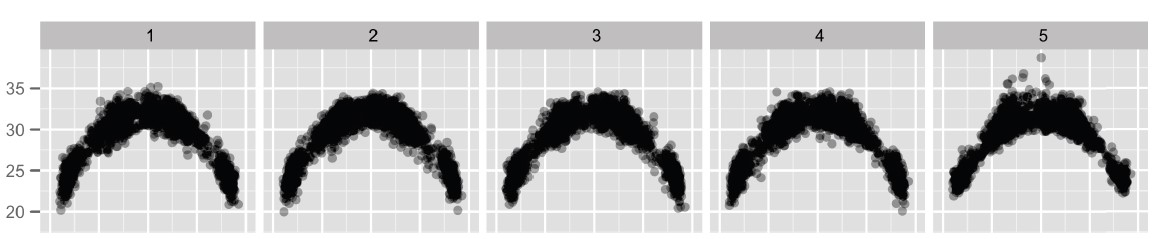
\includegraphics[width=1\linewidth]{ch-visualizer/figures/lineup}
		\caption[A line-up test for $n = 5$. ]{A line-up test for $n = 5$.
			Consistently identifying the raw data against the synthetic data 
			indicates that
			the fitted model may not be good enough. Images from Wickham et al.
			2010~\cite{wickham2010}}
		\label{fig:visualizer:lineup}
	\end{center}
\end{figure}


\subsection{Rejection classification}

So far, we have been discussing classification as black and white, interesting
versus non-interesting. While interacting with the data visually, the user's
concept of what's interesting in the specific dataset may evolve over time; at
the beginning, they have no idea what the data looks like and where to set the
bar for their own standards of dependence. There are several ways to take this
into consideration. 

First, the visualization system could assign a weight to the analyst's responses
by trial number where the last few plots are more valuable than the first few.
However, this may destabilize cases where the user's preferences don’t end up
changing, and it is difficult for the classifier to continuously rebalance each
round given the weights (which, when applied to 2 black and white non-numerical
responses, may also be vague). Secondly, the system can include an alternative
option that allows the user to refuse to label a plot when it's too close to
their decision boundary. This is welcome for the user who is not forced into
making a decision he/she is uncertain about, but it is problematic for the
learner as it causes the hypothesis space to remain unchanged rather than
shrink. The point of the active learning segment is to have the user indicate to
the learner which plots are interesting or not in order to let the computer
better understand their preferences. By allowing for this option, the active
learner may run for too long or return a poorly-defined tree. Finally, there is
a way to consolidate the considerations within each methodology. The system can
contain a third option that permits the user to ``recycle'' the plot. This
allows to user to return to the plot later when he/she has learned more about
what the data looks like and understand their own preferences better, and it
ensures that the active learner will eventually receive data on the ambiguous
plots that it has given the user to label. The main concern is that this could
potentially de-balance an ordering procedure (Section~\ref{***EARLIER
	SECTION***}), but the system can strategically insert the recycled plot 
	between
two plots it differs from with the constraint that the insertion location is
after the current plot.
